\documentclass[11pt,a4paper]{article}

% ========== PACKAGES ==========
\usepackage[
    top=1in,       
    bottom=1in,    
    left=1in,      
    right=1in,     
]{geometry}

\usepackage{amsmath,amsfonts,amsthm,amssymb}
\usepackage{graphicx}
\usepackage{url}
\usepackage{hyperref} 
\usepackage{enumitem} 
\usepackage{booktabs}  
\usepackage{titling}   
\usepackage{lipsum}    % For generating placeholder text (remove if not needed)
\usepackage{fancyhdr}  
\usepackage{array}     
\usepackage{xcolor}
\usepackage{pdfpages}  % For including external PDFs in appendices
\usepackage{microtype}
\usepackage{times}     % Or any other font package if you prefer
\usepackage[backend=biber,style=numeric-comp,sorting=none]{biblatex}
\addbibresource{references.bib}

% ========== TITLE & AUTHORS ==========
\title{\textbf{Efficient Screening in Medical Systematic Reviews: \\
A PhD Progress Report}}
\author{\textbf{Aaron HA Fletcher}\\
Department of Computer Science \\
University of Sheffield \\
\texttt{a.h.a.fletcher@sheffield.ac.uk}}
\date{\vspace{-1em}\small \today}

% ========== PAGE STYLE ==========
\pagestyle{fancy}
\fancyhf{}
\lhead{Efficient Screening in Medical Systematic Reviews: PhD Summary}
\rhead{\thepage}
\renewcommand{\headrulewidth}{0.4pt}

% ========== DOCUMENT BEGINS ==========
\begin{document}
\maketitle
\thispagestyle{empty}

\section*{Executive Summary (1 page)}
Systematic reviews are the cornerstone of evidence-based medicine, guiding clinical decisions by synthesizing extensive research. Yet their creation is resource-intensive: especially the \emph{title and abstract screening phase}, which can consume 10--20\% of total review time~\cite{haddaway_predicting_2019}. My PhD aims to improve \textbf{efficiency} in this screening phase by:

\begin{enumerate}[leftmargin=2em]
    \item \textbf{Exploiting citation networks \& metadata in Continuous Active Learning (CAL).}
    \item \textbf{Developing utility-based stopping criteria} that halt screening once enough \emph{informative} evidence is found.
\end{enumerate}

So far, I have:
\begin{itemize}[leftmargin=2em]
    \item Quantified the \emph{strength} of citation signals in screening: relevant documents more often cite each other than random or irrelevant items.
    \item Explored \emph{utility-based} stopping methods in diagnostic test accuracy (DTA) reviews, finding that a confidence-boundary approach can reduce workload while maintaining high decision agreement.
    \item Demonstrated that more advanced embeddings (BioLinkBERT, etc.) can help ranking, but \emph{gains are modest} if not combined with relational or stopping innovations.
\end{itemize}

\noindent
\textbf{Planned Work:} Evaluate \textbf{Relationship-Prioritized CAL} (leveraging forward/backward citations continuously), \textbf{Graph Neural Network} (GNN) representations (incorporating metadata \& citations), and \textbf{utility-based stopping} across intervention reviews. This approach can significantly reduce resource demands for systematic reviews without undermining their reliability.

\section{Introduction (1 page)}
Systematic reviews are a mainstay of evidence-based medicine, requiring exhaustive searching to identify relevant studies~\cite{ioannidis_mass_2016}. However, the growing volume of biomedical literature inflates the cost of identifying, appraising, and synthesizing evidence~\cite{ghasemi_scientific_2022}. The title and abstract screening stage is a prime candidate for automation because it is typically the most labor-intensive subtask.

\textbf{Continuous Active Learning (CAL)} has been effective in prioritizing relevant studies faster~\cite{cormack_engineering_2016}. CAL repeatedly trains a classifier on labeled examples, ranks the unlabeled pool, and requests user feedback on the highest-ranked items. Despite strong performance, existing methods often treat documents as isolated entities, relying \emph{exclusively} on text-based features. In contrast, \emph{human} reviewers routinely use bibliographic metadata (e.g.\ authors, journals, publication date) and citation networks to guide and expedite screening. 

\textbf{Stopping} is also a crucial component: real reviewers do not always screen an entire pool but instead stop once they have a threshold (often 95\%) of the relevant documents. Yet that threshold is somewhat arbitrary. Many fields, including information science, highlight that \emph{users stop when they have enough information} --- i.e.\ \emph{utility-based stopping}~\cite{ilani_analysis_2024}.

\section{Research Questions (1 page)}
My PhD addresses three main research questions:

\subsection{RQ1: Relationship-Prioritized CAL}
\emph{``What is the impact of integrating citation networks (backward \& forward citations) on CAL performance?''}

I propose adjusting the CAL ranking function to favor documents related to a \emph{known relevant} seed (or seeds). Preliminary experiments confirm that relevant documents cite each other at higher rates than random or irrelevant baselines, suggesting strong potential for \emph{relationship-aware re-ranking}.

\subsection{RQ2: Graph Neural Networks with Metadata}
\emph{``How does incorporating structured metadata (publication date, citation count, etc.) via GNNs affect CAL efficiency?''}

Where RQ1 re-ranks existing scores, RQ2 builds new representations capturing \emph{both} text and relations. Graph Neural Networks (GNNs) pass ``messages'' between connected papers, potentially learning better embeddings. The plan is to train GNN-based representations that fuse textual embeddings from, e.g., BioLinkBERT, with bibliographic metadata.

\subsection{RQ3: Utility-Based Stopping Criteria}
\emph{``How do stopping criteria based on \emph{information utility} compare to classical recall-based thresholds?''}

My initial work in diagnostic test accuracy reviews used a Confidence Boundary approach, halting once the aggregated sensitivity \emph{confidently} met or fell below a predefined threshold. Results showed fewer relevant documents needed while typically preserving the final conclusion. I will generalize these utility-based stopping rules to \emph{interventional} reviews, leveraging known effect sizes and standard errors to detect when additional references are unlikely to change the overall outcome.

\section{Method Overview (2 pages)}
\subsection{Datasets and Preprocessing}
I plan to use the \textbf{CLEF-TAR} datasets (2017--2019)~\cite{kanoulas_clef_2017, kanoulas_clef_2018, kanoulas_clef_2019} and \textbf{Synergy}~\cite{de_bruin_synergy_2023}, which together cover over 150 systematic reviews (mainly medical). Titles/abstracts are available, but references to older or outside documents must be retrieved from external sources like OpenAlex. Preliminary checks show $\approx$80\% coverage in many medical sub-areas; fallback sources (e.g.\ Crossref) are planned if references are missing.

\subsection{RQ1: Relationship-Prioritized CAL (RP-CAL)}
\textbf{Idea:} Boost the rank of any document that is within $n$ hops of a known relevant seed $s$ in the citation graph. Specifically, I multiply the classification score by $(1 + \alpha)$ if the doc is in the seed's forward/backward citation subgraph. 
\[
\text{adjusted}(d) = \text{score}(d)\times \bigl(1 + \alpha\,I_{O_{n(s)}}(d)\bigr).
\]
I will systematically vary $\alpha \in[0,1]$, seeds $\{1,3,5\}$, and compare performance against a standard CAL baseline with no relationship-based re-ranking.

\subsection{RQ2: GNN-Based Document Representations}
I will create a \emph{node} for each document, connected via citation edges, and augment these nodes with textual embeddings (e.g.\ from BioLinkBERT) plus metadata (year, journal ID, etc.). A Graph Convolutional Network (GCN), or Graph Attention Network (GAT), will produce 128--256 dimensional embeddings. These embeddings become the input to a classifier used in CAL. I hypothesize that multi-hop message passing captures deeper relationships, improving recall with fewer documents screened.

\subsection{RQ3: Utility-Based Stopping Rules}
\textbf{Key extension:} In \emph{interventional} reviews, we often see effect measures (mean difference, risk ratio) with confidence intervals. If the 95\% CI for an accumulated effect measure never crosses the clinically meaningful boundary (often zero), screening more documents adds minimal value. Formally, I track the cumulative standard mean difference (SMD) from discovered relevant documents, updating it after each new inclusion. My \emph{confidence-bound} stopping rule halts when:
\[
\text{LB}_k > 0\quad \text{or}\quad \text{UB}_k<0,
\]
assuming zero is the boundary. Meanwhile, classical methods would continue screening until 95\% recall. 

\subsection*{Metrics and Analysis}
\begin{itemize}[leftmargin=1.5em]
\item \textbf{Recall@95\%, R-Precision, WSS@95\%} to measure prioritization performance.
\item \textbf{Percentage of Relevant Documents (PRD)} examined to gauge cost savings.
\item \textbf{Decision Agreement (DA)}: for utility-based stopping, does the final decision match the gold-standard conclusion using all relevant docs?
\item Paired statistical tests (t-tests or Wilcoxon) across multiple systematic reviews.
\end{itemize}

\section{Progress and Preliminary Results (1 page)}
\begin{itemize}[leftmargin=1.5em]
\item \textbf{Citation signals:} A pilot experiment on CLEF 2019 DTA found that relevant documents cite each other at $\approx$28\% rate, compared to $\approx$14--17\% for irrelevant or random seeds. This strongly suggests that leveraging citations early can mitigate CAL’s ``cold start.''
\item \textbf{Encoder-based vs.\ feature-based CAL:} Reproduced prior work~\cite{mao_reproducibility_2024} showing that \emph{large} BioLinkBERT models offer only modest gains in recall metrics over simpler SVM-based approaches. Gains can be overshadowed by hyperparameter choices (batch sizes, selection policy).
\item \textbf{Utility-based stopping for DTA:} My initial conference-submitted paper shows that a \emph{confidence-boundary} method can reduce the proportion of screened relevant documents by 10--20\% at comparable final decisions, outperforming naive fixed-recall.
\end{itemize}

\section{Plan for the Next 12 Months (1 page)}
\begin{enumerate}[leftmargin=1.5em]
    \item \textbf{RP-CAL Experiments (RQ1).} Implement relationship-prioritized re-ranking, vary $\alpha$ and citation depth, evaluate on CLEF-TAR \& Synergy. Target completion: 4 months.
    \item \textbf{GNN-based Document Embeddings (RQ2).} Build adjacency matrices from citation networks + metadata. Compare GCN, GAT, or GraphSAGE to a baseline CAL. Evaluate on same data. Target completion: 4--8 months.
    \item \textbf{Utility-based Stopping for Interventions (RQ3).} Extend confidence-bound approach to effect sizes in intervention reviews. Evaluate \%screened vs.\ decision agreement. Compare to a recall-based baseline. Target completion: 8--12 months.
    \item \textbf{Publications \& Thesis Writeup.} Present results in top-tier IR/NLP/AI venues (SIGIR, ACL), finalize chapters.
\end{enumerate}

\section{University Processes (0.5 page)}
I am on track with all University of Sheffield requirements:
\begin{itemize}[leftmargin=1.5em]
    \item \textbf{Doctoral Development Programme \& CDT Modules:} Achieved results of 64\% (COM61003) and 84\% (COM61004). Additional short courses on HPC usage, advanced Python, and academic writing are completed or planned.
    \item \textbf{Ethics Compliance:} Only re-using \emph{existing}, publicly available data (CLEF, Synergy, OpenAlex). No direct human participation. This approach aligns with Policy Note 9/13 (no further formal approval needed).
    \item \textbf{Data Management:} A dedicated plan ensures consistent file organization, version control (GitHub private repo), and reproducible scripts.
\end{itemize}

\section{Conclusion (0.5 page)}
By incorporating citation networks and metadata into CAL, plus adopting utility-based stopping, this PhD aims to drastically reduce the screening burden in medical systematic reviews. Preliminary findings confirm the potential of both citation-based ranking boosts and utility-driven halts. The next year focuses on systematically evaluating these approaches on multiple datasets and systematically reviewing subtypes. 

\section*{References}
\printbibliography[heading=none]

\newpage
\appendix
\section*{Appendices}
\vspace{-1em}
Below are copies of my completed/in-progress works. These appendices are not counted in the 10-page limit.

\section{Predicting Article Retractions (submitted manuscript)}
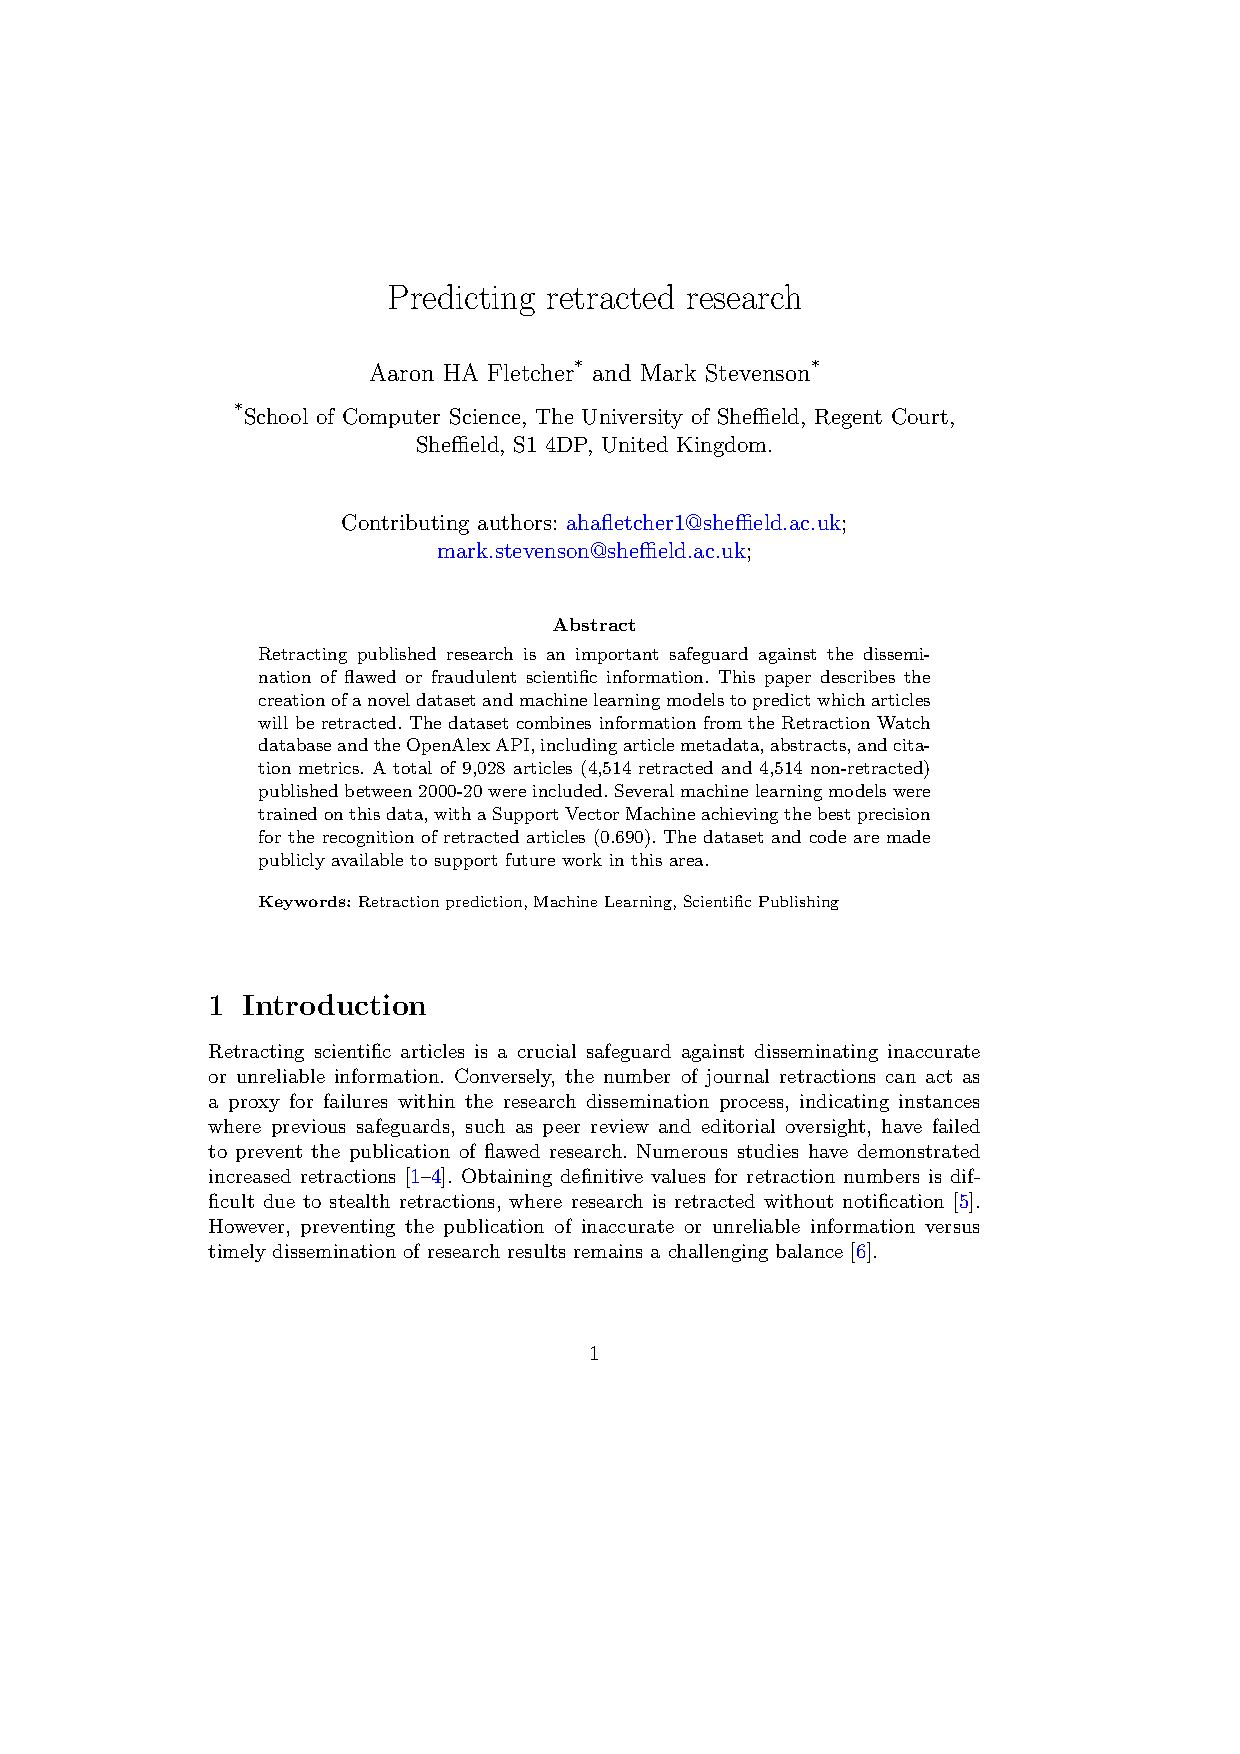
\includepdf[pages=-]{Predicting_Article_Retractions.pdf}

\section{Utility-Based Stopping Methods (submitted manuscript)}
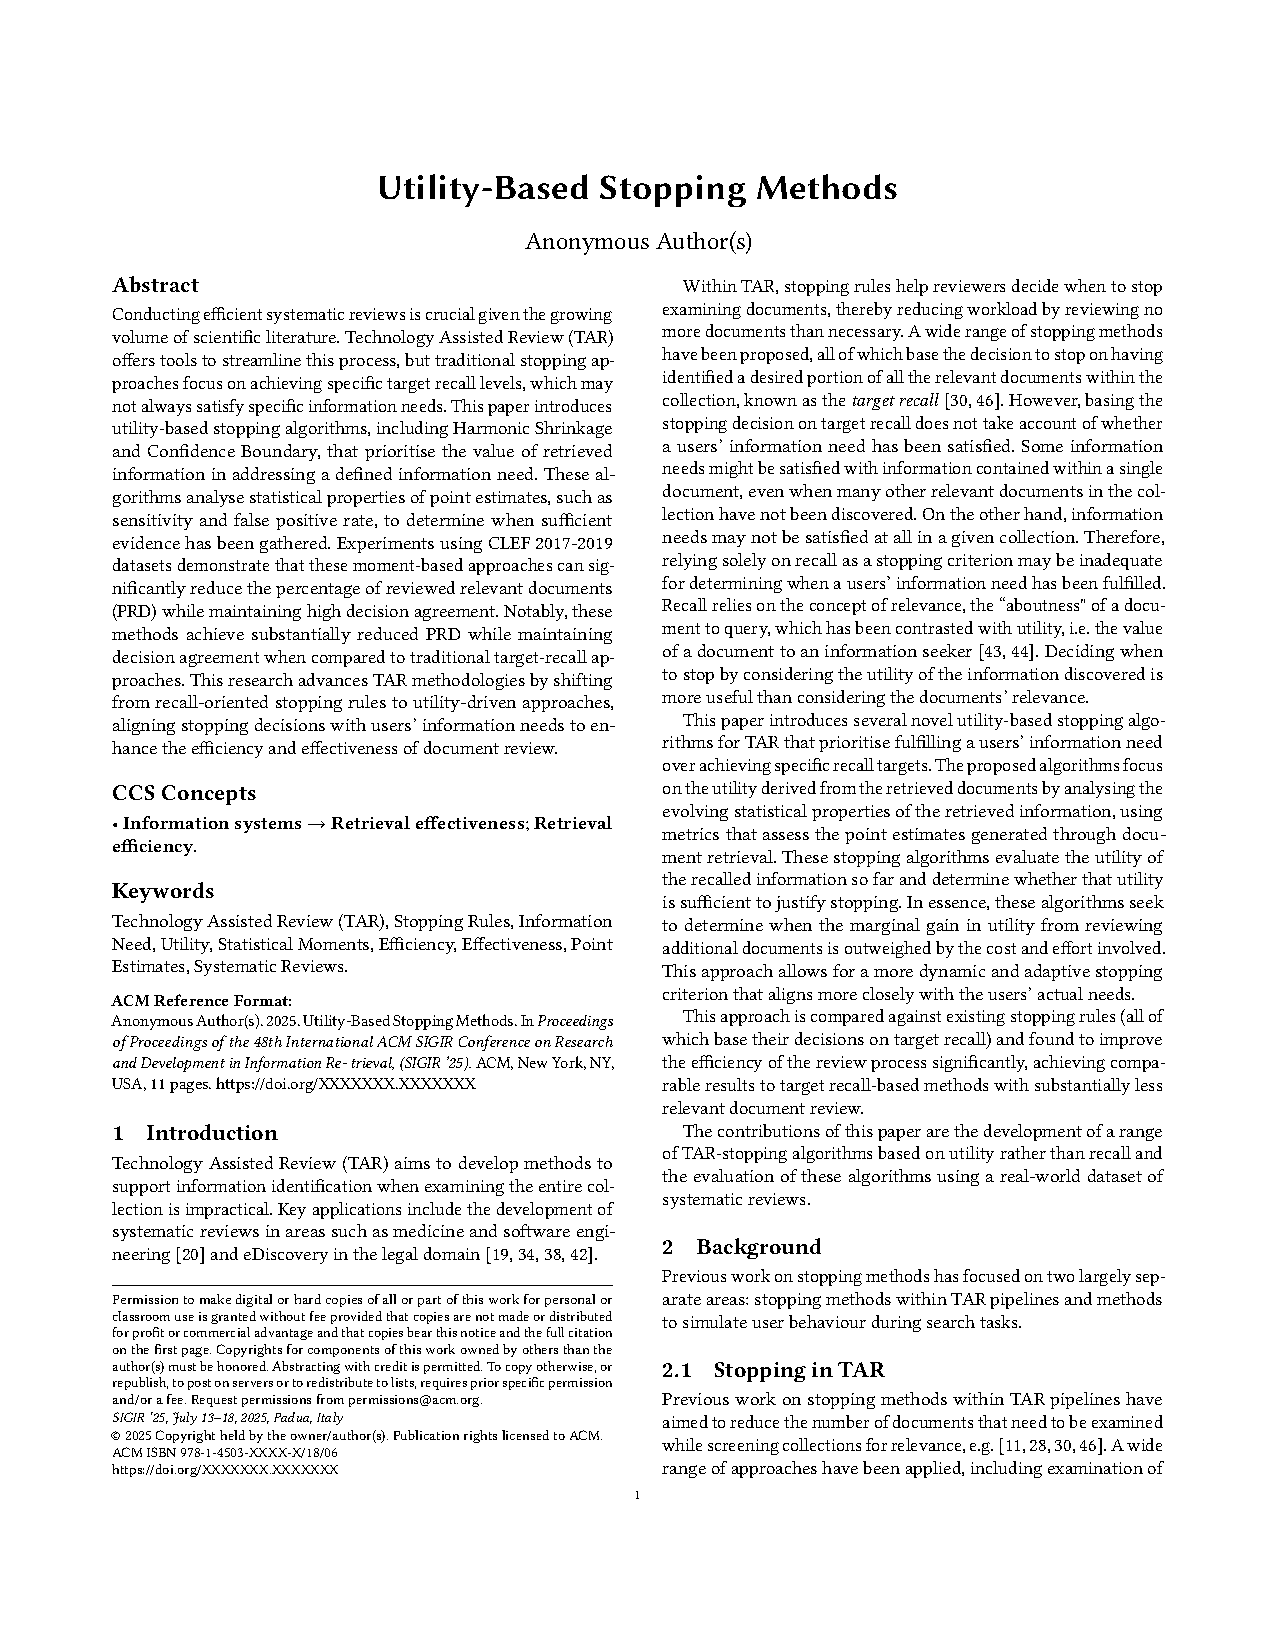
\includepdf[pages=-]{Utility_Based_Stopping_Methods.pdf}

% Add other appendices as needed
\end{document}
